%\documentclass[paper]{geophysics}
\documentclass[manuscript,revised]{geophysics}
%\documentclass[twocolumn,revised]{geophysics}

% An example of defining macros
\newcommand{\rs}[1]{\mathstrut\mbox{\scriptsize\rm #1}}
\newcommand{\rr}[1]{\mbox{\rm #1}}

\newcommand{\psm}{\textit{PSM} }
\newcommand{\twod}{2-D }
\newcommand{\thrd}{3-D }
\newcommand{\bialt}{\textit{BiAlt} }

\newcommand{\correction}[1]{\textbf{\textcolor{red}{ #1}}}
\usepackage{lineno}

% printing options
%\usepackage{pgfpages}
%\pgfpagesuselayout{4 on 1}[letterpaper,border shrink=5mm]


\begin{document}

\title{Refined experimental studies for improving the reduced-scale physical modeling of seismic subsurface measurement}

\renewcommand{\thefootnote}{\fnsymbol{footnote}} 

\ms{version 1.0} % manuscript number

\address{
\footnotemark[1]LUNAM-IFSTTAR, \\
\footnotemark[2]OSUNA \\
\footnotemark[1]LPGN, \\}
\author{Damien Pageot\footnotemark[1]\footnotemark[2], Donatienne Leparoux\footnotemark[1], Mathieu Le Feuvre\footnotemark[1], Olivier Durand\footnotemark[1] and Yann Capdeville\footnotemark[3]}

\footer{Example}
\lefthead{Dellinger \& Fomel}
\righthead{\emph{Geophysics}}

\maketitle

\begin{abstract}

\noindent The potential of experimental seismic modeling at reduced scale has been explored for several years because it provides an intermediate step between numerical tests and geophysical campaigns on field sites. Among the experimental benches using laser interferometry for recording ultrasonic data, the MUSC laboratory is designed as a reliable tool, able to produce experimental seismic reduced scale data from setup involving multi-sources and multi-receivers positions. The recorded signals contain the complete seismic field, suitable for high-resolution imaging techniques like Full Waveform Inversion (FWI). However, experimental seismic modeling uses a point-source and generates 3-D seismic data, whereas most of wave propagation and imaging algorithms make use of \twod forward modeling for numerical cost reasons. Furthermore, geometrical spreading corrections applied on \thrd data become limited in accyracy when geological structures are complex. This leads to inaccurate relative amplitudes between wavefronts which can have an important impact on the quality of the recovered model of parameters. High-resolution imaging methods like FWI are also sensitive to the source waveform: in order to get reliable results, the initial synthetic source must be close enough to the true one, as is the case for the initial model. During the inversion process, the source wavelet can be estimated, either per shot or for the whole dataset, but remains strongly dependent of the initial model, as this estimation will accommodate the discrepancy between the true and current model. In this paper we aim to show the potential of experimental seismic modeling for generating reproducible, realistic and suitable data which can be used as reference for the validation of \twod high-resolution imaging methods.First, we refine the comparison between numerical and experimental data by generating accurate experimental line-sources , avoiding the necessity of geometrical spreading correction for \thrd point-source data. By comparison with 2 D and 3 D numerical modeling based on the Spectral Element Method (SEM), we show the relevance of this approach with respect to published 3D correction methods, in particular when all seismic arrivals are taken into account. Second, we assess the experimental reproducibility of the source emitted in a model by the piezoelectric transducer during a MUSC campaign involving multi-sources multi-receivers acquisition. Both these results refine the accuracy of experimental seismic modeling, and demonstrate that ultrasonic measurement benchs allow to quantitavely reproduce the seismic wavefield. 

%The results of the source estimation through the 2D and 3D experimental setups as well as the reproducibility of the wave-shape contribute to refine the validation of the multi-source and multi-receiver measurement bench as an experimental seismic reduced scale modeling system and prove the capacity of ultrasonic devices used, associated to the positionnment bench to perfectly and quantitatively reproduce the seismic surface measurements and the complete wave-field involved.
\end{abstract}

\modulolinenumbers[5]
\linenumbers

% ## INTRODUCTION
\section{Introduction}

% #### Nature and scope of the problem

\noindent Since the early developments of seismic imaging methods in the middle of 20th century, several approaches and algorithms innovations have been proposed. The improvements deal with both the qualitative imaging techniques like migration (e.g. \citet{Berkhout_MSS_2012,Guofeng_GPU_2013}), novel applications of quantitative imaging methods such as the first arrival tomography (e.g. \citet{Bohm_CWS_2015}), or even more recent approaches like the Full Waveform Inversion (e.g. \citet{Perez_AWI_2014}, see \citet{Virieux_FWI_2009} for a revue of this last decade). These refinements are proposed at different application scales, from near-surface civil engineering topics to global crustal imaging, and including oil prospection. Validation is generally done by the use of well known shared benchmark like the Marmousi model \citep{martin2006marmousi2}. However, the synthetic data are generally computed using the same wave propagation modeling engine used in the inverse problem process. This  approach, called \textit{inverse crime} \citep{Wirgin_TIC_2004} is particularly useful for validating an algorithm in its early development stage but does not take into account the artifacts associated to the assumptions of the forward problem. In the other hand, it is often challenging to assess the accuracy of a given method from real experiments, lacking precise information about the Earth's interior which can lead to geological misinterpretation \citep{Morozov_ARF_2004}. In this context, controlled experimental measurements appear as a powerful intermediate step, providing they are capable of producing accurate data.

\noindent Physical Small Scale Modeling Methods (\psm). \psm has been used for several decades to study the propagation of waves in media presenting different levels of complexity, ranging from acoustic wave propagation in homogeneous media to elastic wave propagation in \thrd heterogeneous anisotropic media. This experimental approach has been used at first to describe the phenomenology of propagating waves (for example  Rieber, Howes). In a second phase, PSW has allowed to test imaging processes (Hiltermann, French, Bishop, pratt, Isaac), or validate numerical tools \citep{Favretto_NMT_2013}. For these different works, the technology used has become more and more sophisticated. Nowadays most of experimental benches include piezoelectric transducers to simulate multi-sources and multi-receivers \citep{Wong_SPM_2009} or immersed zero-offsets profiles \citep{Favretto_NMT_2013}. Laser interferometry is a recent alternative, providing seismic records free of coupling effects, in solid media (Bodet, Van Wijk, Bretaudeau 2011,2013), or in gelee ( ). All the above studies have shown the relevance of experimental seismic data obtained under controlled conditions. However, key points needs to be adressed in order to quantitatively simulate seismic surface measurements generated with a hammer fall source: first, the modeling of surface waves prevent the use of immersed media, and second, the omni-directionality of the radiation pattern implies a physical source point. To this end, the MUSC (Mesures Ultrasonores Sans Contact in french) system has been designed \citep{Bretaudeau_SSM_2011} to simulate (1) wide-angle on-shore acquisitions modeling both body waves and surface waves, (2) automatic multisource-multireceiver measurements with a high-productivity, (3) high-precision source-receiver positioning and (4) high-precision recording of absolute surface displacement without coupling effects. 

\noindent These abilities have been validated  experimentally on a 3D small-scale model  containing a cavity \citep{Bretaudeau_SSM_2011}. The comparison with 2D numerical modeling showed sharp similarities on the diffracted and converted arrivals, after accounting for the experimental source waveform. Since the numerical source was simulated in 2D, some corrections were required to compare the resulting amplitudes, leaving moderate discrepancies that are discussed in \citet{Bretaudeau_SSM_2011}. 

%\noindent The source diagram was assessed with a parallel measurement bench, showing an omni-directional propagation. % but the repeatability of the source impact was not studied.

%\noindent In general, numerical modeling implicitely use line-source in 3D-space, because 1) 3D elastic wave propagation is computationaly expensive and 2) imaging methods assume that media are invariant in the third dimension. For this reason, the differences between 2D and 3D propagated wavefields must be explicitely take into account to successfully validate imaging methods using field or experimental data. 

\noindent 3D elastic wave propagation modeling methods are computationaly expansives and imaging methods are used mainly for 2D structures. Therefore, forward problems implicitly use line-source in 3D-space while field and experimental data are acquired using punctual sources which produce 3D wavefields. For this reason, the differences between 2D and 3D propagated wavefields must be explicitely take into account to successfully validate imaging methods using field or experimental data. 

%\noindent This differences between 2D and 3D propagated wavefields must be take into account to successfully validate imaging methods using field or experimental data.

\noindent For this purpose, a widely used method consists in performing spreading transformations of 3D-wavefield for 2D-media as a pre-processing step. Several 3D-to-2D transformation techniques have been proposed, each under the assumption that the medium is either 1D, or 2D but invariant along the axis perpendicular to the strike direction.

\noindent Recently, \citet{Forbriger_LSS_2014} proposed the \textit{hybrid} method which makes it possible to correct geometrical spreading with a good accuracy for both near- and far-field data. This method, described in a following section, is used in this study to compare experimental and numerical data. 

\noindent Another critical point for high-resolution imaging methods is the knowledge of the source time function, generally treated as an unknown parameter in the case of field data. A good approximation of the source excitation allows to avoid source wavelet estimation during the inversion process and to facilitate the validation of the imaging method. This source time function is easily estimated from experimental data, further supporting PSM for the validation of seismic imaging methods.

% #### State the objectives
\noindent Our objective here is to complete the validation of the capability of ultrasonic devices to precisely and quantitatively simulate surface seismic data carried out with multi-sources and multi-receivers setting. This quantitative refined approach will increase the potential of the MUSC laboratory as a reliable tool for generating experimental data which will be distributed in the scientific community and used as references for validation of seismic imaging methods.

%\noindent In this study, we refine the validation of the MUSC laboratory, in order to emphasize its potential for providing accurate experimental data to the scientific community.

\noindent In this way, we further present two experimental studies in order to : 1) refine  the comparison between numerical and experimental data by taking into account the 3D/2D geometrical spreading effects through an alternative way that we compare to the corrections proposed in the literature ; 2) identify the reproducibility of the source impact and, consequently, the data repeatability, and estimate source time functions usable for 2D imaging methods. These approaches will complete the knowledge of the system and facilitate the achievement of massive multi-source and multi-receiver data simulating subsurface seismic experimental campaigns. Moreover, they provide quantitative informations about the data quality for geophysicists who need to use them measurement based on reduced scale models. 

% #### Describe the method of investigation
%\noindent In order to achieve these objectives, we used a seismic wave modeling code based on the Spectral Element Method \citep{Komatitsch_SEM_1998,Komatitsch_ISM_1999,Komatitsch_SEM_2005,Festa_PML_2005} to provide numerical signals as reference data for comparison. 

% #### Describe the principal results of the investigation

\noindent The numerical characteristics of the code used are described in a first part below. Afterwards, the specificities of the MUSC laboratory are explained, followed by the presentation of the models used. Finally The two coupled studies on experimental data are detailed, in the respective aims (1) of refining the comparison between numerical and experimental data by taking into account the geometrical spreading effects between \twod and \thrd data through an alternative way, and (2) of identifying the reproducibility of the source impact to validate the data reproducibility.


% ## METHODS
\section{Methods}

% #### Spectral Element Method
\subsection{Numerical modeling: Spectral Element Method}

\noindent For this study, we need a numerical modeling method which has a spatial discretization convenient for the representation of complex environments and provides high precision results as well as low numerical dispersion. Thus, we use the Spectral Element Method (SEM) for two-dimensional and three-dimensional elastic wave propagation modeling \citep{Komatitsch_SEM_1998,Komatitsch_ISM_1999,Komatitsch_SEM_2005,Festa_PML_2005}. 

\noindent The SEM is a variant of Finite Element Method (FEM) \citep{Lysmer_FEM_1972,Seron_FEM_1990,Hulbert_FEM_1990,Tromp_SEM_2008} based on a high-order piecewise polynomial approximation of the weak formulation of the wave equation which leads to a spectral convergence ratio as the interpolation order increases. Considering near-surface experiments, one advantage of SEM is that the weak formulation naturally satisfy the free-surface condition which allows to simulate surface wave propagation with a great accuracy \citep{komatitsch1998spectral,komatitsch1999spectral,Komatitsch_SEM_2005}. Contrary to FEM, which have a variety of available element geometry \citep{dhatt1984finite}, SEM is limited to quadrilateral elements in 2D and hexaedral elements in 3D. Note that SEM on tetrahedral elements exists \citep{komatitsch2001wave} but leads to theoretical complications. However, quadrangle and hexaedra are well suited to handle complex geometries and interface matching conditions \citep{Cristini_SEM_2012}. 

\noindent In SEM, the wave-field is expressed in terms of high-degree Lagrange interpolants and the integrals calculation are based on the quadrature of Gauss-Lobatto-Legendre (GLL). Each element is discretized with Lagrange polynomials of degree $n_{l}$ and contains $n_{l}+1$ GLL points which constitute their local mesh. This combination of high-degree Lagrange interpolants with the GLL quadratic integration leads to a perfectly diagonal mass matrix which provides in turn a fully explicit time scheme suitable for numerical simulations on parallel computers \citep{komatitsch1998spectral,komatitsch1999spectral}.

\noindent The spatial resolution of SEM is controlled by the typical size of an element ($\Delta h$) and the polynomial degree in use on an element ($n_{l}$). Typically, a polynomial degree $n_{l}=4$ are optimal for seismic wave propagation modeling \citep{moczo2011finite} even if $n_{l}=8$ stay numerically affordable in 2D. For accurate results, required $\Delta h$ is of the order of $\lambda_{min} /2 < \Delta h < \lambda_{min}$ for $n_{l}=4$ and $\lambda_{min} < \Delta h < 2\lambda_{min}$ for $n_{l}=8$, $\lambda_{min}$ being the smallest wavelength of waves propagated in the model. The time marching scheme is governed by the stability CFL condition:

\begin{equation}
	\Delta t < \mathcal{C}\frac{\Delta h}{c_{max}}\,   
\end{equation}

\noindent where $\mathcal{C}$ is the Courant constant and $c_{max}$ is the maximum wave velocity, typically the P-wave velocity. The Courant constant $\mathcal{C}$ is determined empirically, depending on the application, and is fixed to a maximum of 0.30 for this study.

\noindent In our study, the models are meshed with quadrangles (2D) and hexaedras (3D) using the open-source software package GMSH \citep{Geuzaine_MSH_2009}. 


% #### MUSC bench
\subsection{Physical modeling: MUSC laboratory}

\noindent The MUSC laboratory \citep{Bretaudeau_SSA_2008b,Bretaudeau_SSM_2011,Bretaudeau_FWI_2013} is built to experimentally reproduce low noise field seismic data on reduced scale model. Figure \ref{panel_musc_bench} shows the measurement bench and its components : it is composed of a honeycomb tab and two arms which control the source and the receiver positions with a precision of 10 $\mathrm{\mu m}$.

\noindent The receiving system of MUSC laboratory is a laser interferometer based on the phase shift of the reflected laser signal due to the particular displacement at the surface of the model during the seismic waves propagation in the medium. The diameter of the laser beam on the model surface equals 20 micrometers for the focal distance of 40 mm and makes it possible a detection of a vertical displacement of the order of the nanometer in the frequency range from 10 kHz to 20 MHz. The laser interferometer constitutes a non-coupled receiver which avoids the complicated modeling of the coupling effects on measurement.

\noindent The seismic source in the MUSC laboratory is simulated by a piezoelectric transducer linked to a launching and synchronization system. It allows to choose the source function, i.e., a waveform like a Gauss or Ricker function, for a central frequency $f_{0}$ and a time delay $t_{0}$. For that, the source is generated by a waveform generator and is then amplified before being transmitted to the small-scale-model.

\noindent Since the wave equation is linear, the change of scale must keep the relationship between observables, i.e. amplitudes and time arrivals. About the amplitude, the quality factor $Q$ is chosen to be in the same range as the materials of near surface. For the time scaling, the key parameter is the ratio between the propagated seismic wavelength and the spatial dimensions of the experience which includes the model geometry, the spatial increment between the sources and the receivers positions, but also the dimensions of the source impact. In the framework of seismic physical modeling, the latter must be as close as possible to a point source in order to simulate the spatial energy radiation pattern of a weight drop on the surface, i.e. with an omnidirectional emitted P-wave.

\noindent In the MUSC laboratory, the main frequency bands used for reduced scale data are [ 20 kHz ; 200 kHz] and [ 300 kHz; 800 kHz], respectively called here "low frequency band" and" high frequency band". For the lower spectral band, a commercial piezoelectric transducer is used without any coupling gel. For the higher band, the piezoelectric source is coupled through a conical adapter which is sticked to the transducer in order to obtain the expected impact surface. The resulting radiation patterns of the sources are constantly nearly omni-directional for the range of recorded frequencies (see \citet{Bretaudeau_SSM_2011} for details).

\noindent The lower frequency band is well adapted to simulate seismic experiment applied to near surface through the scales ratios proposed in tables 1 and 2. In the first case (table 1), a central frequency of 100 kHz in the laboratory corresponds to a central frequency of 100 Hz on the field, whereas in the second one (table 2) a central frequency of 100 kHz in the laboratory corresponds to a central frequency of 50 HZ on the field. Note that with these propositions, the  quality factor $Q$ and the density $\rho$ are modeled with a ratio equal to 1, i.e. they remain the same at both of the scales. Actually small-scale models are generally made of thermoplastic or casting epoxy resin materials \citep{Bretaudeau_FWI_2013}.The mechanical properties of these materials provide attenuation characteristics close to natural soil materials of subsurface media. Their seismic velocities are about 2 times of those in subsurface materials as proposed in table 2. The possibilities of combinations can generate the impedance contrasts encountered in the geophysical issues. 

\noindent The MUSC bench presented above has been studied for simulating with a great reproducibility the typical field campaigns of subsurface seismic measurement. The validation was achieved by comparison between small scale measurement and numerical data \citep{Bretaudeau_SSM_2011}. Results have shown a great reproducibility of the converted and diffracted events recorded on the vertical component. The amplitudes analysis had been conducted through 2D-3D corrections and small discrepancies remained due to the difficulty of taking into account the S and P waves in the same way. For this reason, we propose here to refine the study by testing a more recent correction methodology \citet{Schafer_LSS_2014} as well as providing experimental and numerical, 2D and 3D data. This approach will be achieved through data carried out on two models that are presented below.


% ## Models
\subsection{Characteristics of the scale models tested}

\noindent In this study, we consider two different reduced scale models. The first one is homogeneous whereas the second one contains a deeper layer with a geometrical variation of the interface along the profile. The top layer, as well as the entire first model, is made of epoxy-resin called F50. The deeper layer is built with a more dense resin called LAB1000. Latter model is named \bialt. The specific properties of these two kinds of resins are summarized in the table 3. As required, note that the Q-factor values are of the same order of the Q-factor value in the shallowest parts of some natural media.

\noindent As described in the previous part and proposed in table 2, it is possible to take into account a scale ratio equal to 2 between real and reduced model velocities, makes it possible to use a 100 kHz Ricker source in order to simulate a 50 Hz Ricker source in reality, which is realistic for simulating an hammer impact on the surface. In this case, the distance scale ratio is 1000 such that a 1 mm distance in the laboratory experiment corresponds to a 1 m distance in reality. 

\noindent In a next section, the recorded signals will be finely analyzed for a maximum offset equal to 60 mm in the case of the homogeneous model and 100 mm for the \bialt model. Thus, the resin models have to be wide enough in order to carry out this receiver-source distances without providing boundary echoes which could interfere with the direct arrivals. For that, the homogeneous model is 500 mm long and 504 mm large and 115 mm high. The \bialt model is 540 mm long, 300 mm large and 203 mm high. The geometry is presented in figure 3 and simulates an interface between a 3 m thick layer of clay overcoming a limestone layer.

\noindent The numerical meshing required for numerical simulations involve dimensions of cells about $e_{s}<3.43\ mm$ for F50 material and $e_{s}<4.66\ mm$ for the LAB1000 material, considering a polynomial degree $n_{l}+1=5$ and a slightly over-estimated maximum frequency $f_{max}=300\ kHz$ for $f_{0}=100\ kHz$. The resulting meshing structure for the \bialt model is presented figure \ref{panel_bialt_mesh}.

\noindent These two resin blocks as well as their corresponding numerical models will be used for generating seismic data with punctual sources and line sources, for the homogeneous model, in order to study the effective source excitation emitted in the MUSC bench and its reproducibility.

\subsection{3D/2D differences}

\noindent Most of seismic imaging methods implement a 2D forward problem, essentially for numerical cost reasons. It results in an implicit use of 2D line-source, invariant along the direction perpendicular to the strike direction, while field data are generally acquired using point-source (hammer-blow, mass). Consequently, it exists differences in amplitude and phase between point-source and line-source responses which must be considered in the case inversion of field data with a 2D imaging method.  

\noindent The displacement field $u$ can be evaluated at general position and time $(\mathbf{x},t)$ by \citep{aki2002quantitative}:

\begin{equation}
	u(\mathbf{x},t) = \int_{-\infty}^{+\infty}d\tau \int \int \int_{V} G(\mathbf{\xi},t-\tau;\mathbf{x},0)f(\mathbf{\xi},\tau)dV(\mathbf{\xi})\ ,
	\label{eq:displacement}
\end{equation}

\noindent where $G(\mathbf{\xi},t-\tau;\mathbf{x},0)$ is the Green's function and $f(\mathbf{\xi},\tau)$ is the seismic source function. The body force distribution for a point source $f_{P}$ and a line source ($f_{L}$) for a 2D structure $G(\mathbf{\xi},t-\tau;\mathbf{x},0)$ invariant along y-axis at position $ \mathbf{x_{s}}=(x_{s}, y_{s},z_{s}) $ are:

\begin{eqnarray} 
	f_{P}(\mathbf{x},t;\mathbf{x_{s}})=\mathbf{F}(t)\delta_{\mathbf{x}}(x-x_{s})\delta_{\mathbf{x}}(y-y_{s})\delta_{\mathbf{x}}(z-z_{s})\ , \label{eq:point-force} \\
	f_{L}(x,y,z,t;x_{s},z_{s})=\mathbf{F}(t) C \delta_{\mathbf{x}}(x-x_{s})\delta_{\mathbf{x}}(z-z_{s})\ , \label{eq:line-force}
\end{eqnarray}

\noindent Substituting equation \ref{eq:point-force} in equation \ref{eq:displacement} and equation \ref{eq:line-force} in equation \ref{eq:displacement} lead to the wave motion due to a point-source $u_{P}$ and the wave motion due to a line-source $u_{L}$ 

\begin{eqnarray}
	u_{P}(\mathbf{x},t;\mathbf{x_{s}})=\int_{-\infty}^{+\infty}\ G(\mathbf{x_{s}},t-\tau;\mathbf{x},0)F(\tau)d\tau, \label{eq:point-displacement} \\
	u_{L}(x,y,z,t;x_{s},z_{s})=\int_{-\infty}^{+\infty} \int_{-\infty}^{+\infty} G(x_{s},y',z_{s},t-\tau;\mathbf{x},0)F(\tau)Cdy'd\tau\ , \label{eq:line-displacement}
\end{eqnarray}

\noindent The equivalent displacement $u_{L}$ for a line-source can be obtain from the displacement field $u_{P}$ generated by a point source by integration along $y$:

\begin{equation}
	u_{L}(x,y,z,t;x_{s},z_{s})=\int_{-\infty}^{+\infty}u_{P}(x,y,z,t-\tau;x_{s},y',z_{s},0)Cdy'\ .
	\label{eq:line-point-relation}
\end{equation}

\noindent Latter means that in term of amplitude, the displacement generated by a line-source is greater than displacement generate by a point-source.
 
\noindent Taking $g_{k}^{3D}(r)$ and $g_{k}^{2D}(r)$, the Fourier transform of the 3D and 2D Green's function in the acoustic approximation, respectively, with $k$ the wavenumber and $r=|\mathbf{x}-\mathbf{x_{s}}|$ the source-receiver offset. In the far-field approximation, \citet{Forbriger_LSS_2014} demonstrate:

\begin{equation}
	\lim\limits_{r \rightarrow \infty} \frac{g_{k}^{2D}(r)}{g_{k}^{3D}(r)}\approx \sqrt{\frac{2\pi r}{k}}.e^{i\frac{\pi}{4}}\ .
	\label{eq:far-field-frac}
\end{equation}

\noindent Replacing the wavenumber $k=\omega/v_{ph}$, where $\omega$ is the angular frequency and $v_{ph}$ is the phase velocity, it results:

\begin{equation}
	\sqrt{2\pi r v_{ph}}.\sqrt{\frac{\pi}{\omega}}e^{i\frac{\pi}{4}}=F_{amp}.\widetilde{F}_{\sqrt{t^{-1}}}\ ,
\end{equation}

\noindent where $F_{amp}$ is the amplitude factor and $\widetilde{F}_{\sqrt{t^{-1}}}$ applies the phase shift. It results in:

\begin{equation}
	u_{L}(r,\omega)=u_{P}(r,\omega).F_{amp}.\widetilde{F}_{\sqrt{t^{-1}}}\ .
	\label{eq:single-velocity}
\end{equation}

\noindent This correction is called the \textit{single-velocity} transformation which is recommanded for small offset. For larger offset, stating that offset is almost equal to the propagation distance, \citet{Schafer_LSS_2014} propose to replace the previous amplitude factor with:

\begin{equation}
\label{eq:direct-wave}
F_{amp}=r\sqrt{\frac{2 \pi}{t}}\ .
\end{equation}

\noindent The resulting correction is called the \textit{direct-wave} transformation. Finally, the \textit{hybrid} transformation proposed by \citet{Forbriger_LSS_2014} and \citet{Schafer_LSS_2014} consists to use both previous transformation with smoothly offset conditioned transition from near-field to far-field.

\noindent The \textit{hybrid} method was successfully validated by \citet{Schafer_LSS_2014} in terms of modeling and reconstruction tests with a 2D FWI method and 3D numerical data generated in a 2D structure. Given its performance, the \textit{hybrid} is used in the next sections for comarisons with experimental data. 

\section{Results}

% #### From point-source to line-source acquisition
\subsection{From point-source to line-source response}

\noindent The approach detailed here consists in generating data with a 2D line-source as well as a 3D point-source and analyzing the similarity to numerical results under the same conditions. This is conducted to answer to two needs : 1) the quantitative refined validation of the reduced scale data , 2) the validation of the reduced scale data as a 2D set which is intermediate between numerical simulation and field data suitable for the 2D imagery tests . Indeed, in the framework of wave propagation modeling and imaging methods, even if \thrd acoustic algorithm exists \citep{benhadjali_FWI_2008,plessix_FWI_2010} and \thrd elastic algorithm are always in development \citep{castellanos_AMD_2011,Borisov_FWI_2015}, most of available algorithms are limited to the \twod elastic and \thrd acoustic approximation especially for computational cost causes. More, a widely used way to validate imaging methods consists in inverse crime while the validity of applications on real dataset is conditioned by strong \textit{a priori} and a weak knowledge of the target. All of these leads to a limited validation of the efficiency of imaging methods to recover parameter models. Thus, it is critical for \twod inversion of field data to accurately correct the difference between \twod and \thrd geometrical spreading.

%\noindent Point-source data can be corrected from geometrical spreading using a simple two-steps signal processing: (1) convolving each trace by $\sqrt{t^{-1}}$, where $t$ is the time, to correct the phase shift of $\pi/4$ and (2) applying a taper $\sqrt{t}$ to all traces to correct relative amplitudes. Some variation exist, for examples, using a linear source wavelet estimation method to correct the phase \citep{Bretaudeau_FWI_2013} or applying an offset conditioning to obtain a better correction of amplitudes \citep{Tran_SWT_2013}. To correct some biases of these methods, \citet{Forbriger_LSS_2014} and \citet{Schafer_LSS_2014} have introduced, and successfully applied to synthetic data, the \textit{hybrid method}. 

%\noindent In the \textit{hybrid method} the geometrical spreading correction is conditioned by: (1) the offset, (2) the knowledge of the wave propagation velocities in the medium and (3) a user defined ratio used to smoothly correct amplitudes from near offset, which used the direct wave correction factor (eq. \ref{eq:direct-wave}), to far offsets, which used the single velocity correction factor(eq. \ref{eq:single-velocity}): 

%\begin{equation}
%	\label{eq:direct-wave}
%	F_{amp}=r\sqrt{\frac{2}{t}}\ ,
%\end{equation}

%\begin{equation}
%	\label{eq:single-velocity}
%	F_{amp}=\sqrt{2rv_{phi}}\ ,
%\end{equation}

%\noindent where $o$ is the source-receiver offset, $t$ is time and $v_{phi}$ is the phase velocity. 

%\noindent The \textit{hybrid} method is efficient but difficult to calibrate without reference data. Moreover, the correction are derived from far-field acoustic approximation. Then, results are thus strongly dependent of user's \textit{a priori} and attempts. Moreover, this kind of signal correction is mostly valid for one-dimensional medias, two-dimensional ($x,z$) medias invariant along the $y$-axis.    

\noindent The \textit{hybrid} method, presented in the previous section, is an efficient spreading transform which makes it possible to reconstruct velocity models with 2D-FWI method using 3D-data. However, this method is derived from a far-field acoustic approximation of Green's functions and is known to fail for back-scattered surface wave \citep{Schafer_LSS_2014}. Moreover, the correct smooth transition between \textit{single-velocity} and \textit{direct-wave} transformations is not easy to determine without 2D reference data. This is the case for both field and experimental data and the spreading transformation results become strongly dependant of the user's attempts and experience.
 
\noindent Thus, the missing step between purely numerical validation and real data applications can be addressed by an alternative approach that consists in recording experimental seismograms generated by line-sources under controlled conditions. Here, we take advantage of the experimental framework to explore this alternative approach specific through the MUSC laboratory, \textit{i.e.} caring out 2D measurement from 2D source-lines. Figure \ref{amplitude_acqui_principle} shows a schematic representation of the principle for this kind of experiment. The line-source is composed of a finely-sampled line of point-source and a line of receiver for each considered offset. 
 
\noindent Taking advantage of the reciprocity principle in case of a vertical source and a vertical component recording, the experiment can be simplified by considering only one receiver per offset, on a line perpendicular and centered to the defined line-source. All traces of each common receiver gather are then stacked together to obtain the line-source response. In order to apply this protocol, we have to choose a suitable sampling interval $\Delta s$ between each point-source constituting the pseudo line-source to ensure applicability of the \textit{Huygens principle}. Given the material properties of $F50\ pure$ epoxy-resin, we choose an interval $\Delta s=\lambda_{min}/10 \tilde{=}0.5\ mm$ over a line of $300\ mm$ long which leads to 601 point-source positions.

Four receiver positions are available: 45, 50, 55 and 60 mm offset. The source time function (for the numerical simulation as well as for the experimental test) is a Ricker, the second derivative of a Gaussian:

\begin{equation}
	s(t) = (1-2(\pi f_{0}(t-t_{0}))^{2})~e^{-(\pi f_{0}(t-t_{0}))^{2}}~,
	\label{eq:ricker-source} 
\end{equation}

\noindent where $f_{0}$ is the central frequency and $t_{0}$ is the peak time. Here, we take a central frequency $f_{0}=100\ kHz$ and $t_{0}=0.03\ ms$. The obtained data set are filtered using a low-pass Butterworth filter with a cutoff frequency $\omega_{c}=250\ kHz$ to remove noise and are tapered at the beginning using a cosine taper function of width $w=0.03\ ms$ on the time signal. The experimental line-source data is obtained through a weighted stack over common offset traces. Figure \ref{amplitude_stack_principle} shows the results for both numerical simulation and experimental data. The signals emitted by a line of point-sources and recorded at the first receiver position (45 mm) are presented in figures \ref{amplitude_stack_principle}(a,c) for the numerical and experimental tests respectively.  Note there is no attenuation accounted for the numerical modeling, so we do not compare directly numerical and experimental results. Moreover, all the resulting traces are normalized to be comparable to the experimental tests. The numerical result (fig \ref{amplitude_stack_principle}(a)) clearly shows the direct attempted P and S wavefronts and the reflected PP and P-SV wavefronts as mentioned (labels $1$, $2$, $3$, $4$ on figure \ref{amplitude_stack_principle}). These similarities between numerical simulation and experimental data are altered by multiple echoes visible on experimental data (labeled E on figure \ref{amplitude_stack_principle}(b)), as a ringing effect on the source wavelet due to the piezoelectric transducer coupling on the model surface. This point will be addressed in the next section focused on the source reproducibility.   

\noindent The comparisons of point-source and line-source data, at the first receiver position (45 mm offset), are presented in figures \ref{amplitude_stack_principle}(b) and \ref{amplitude_stack_principle}(d), respectively for numerical and experimental tests. To complete the comparison, a 2D modeling result is added in figure \ref{amplitude_stack_principle}(b) as a reference.

\noindent First, figure \ref{amplitude_stack_principle}(b) shows that 3D line-source data (green line) and 2D data (blue line) are perfectly superimposed until 0.18 ms, afterward the PSv amplitude (\textit{i.e.} the last arrival) is abnormally high for the 3D line-source data. As shown in equation \ref{eq:line-point-relation}, a line-source is a sum of an infinite number of point-source along an axis. Here, the experimental 3D setup, which have finite dimensions in space, can be the cause of this amplitude difference.

\noindent Nevertheless, the global adequation between numerical data highlights the validity of sampling a finite line-source by a set of point-sources but is subject to some boundary effects.

\noindent Second, even if for experimental results some differences in waveforms are visible between 0.08 ms and 0.10 ms, in both numerical (figure \ref{amplitude_stack_principle}(b)) and experimental (figure \ref{amplitude_stack_principle}(c)) cases, the comparison of 3D point-source and 3D line-source data show the expected phase shift of $\pi/4$ (equation \ref{eq:far-field-frac}).

\noindent Similar comparisons, for the four source-receiver offsets, are shown in figures \ref{panel_amplitude_sem}(a) and  \ref{panel_amplitude_sem}(c) for numerical and experimental data, respectively.

\noindent In order to test the improvement of our approach to provide 3D line-source data in comparison to spreading transformation methods, our results are compared to data obtained using the \textit{hybrid} method. Figures \ref{panel_amplitude_sem}(b) and  \ref{panel_amplitude_sem}(d) present the comparison between 3D line-source data and transformed 3D point-source data.

\noindent The comparison of numerical results (figure \ref{panel_amplitude_sem}(b)) shows that the \textit{hybrid} method is able to produce line-source data with a very good agreement  in terms of both amplitude and phase. However, PP and PSv reflected waves (back-scattered wave) remain likely different.

\noindent The same comparison is done for experimental data in figure \ref{panel_amplitude_sem}(d). This last result also shows a good agreement between 3D line-source  and transformed 3D point-source data up to 0.12 ms (mainly direct-waves). However, discreapencies occur for the reflected waves. The first reflected wave is marked by a red line in figures \ref{panel_amplitude_sem}(b) and \ref{panel_amplitude_sem}(d).
 
%\noindent The comparisons of the point-source and line-source responses are presented in figures \ref{amplitude_stack_principle}(b) and \ref{amplitude_stack_principle}(d), respectively for numerical and experimental modeling. Here, the point-source response (red line signals in the figures) corresponds to the central trace (distance $0\ mm$) visible on figures \ref{amplitude_stack_principle}(a) and \ref{amplitude_stack_principle}(c) and the equivalent line-source response (green line signals) is the weighted stack of all traces shown on the same figures (\ref{amplitude_stack_principle}(a,c)).  An other reference is taken into account for numerical modeling, i.e. we provide a line-source response from \twod modeling (blue line signal in figure \ref{amplitude_stack_principle}(d)) for a comparison of both \thrd and weighted stack results. First, figure \ref{amplitude_stack_principle}(b)) shows that the two numerical reference signals are not distinguishable : the blue and green lines signals are perfectly superimposed until 0.18 ms, afterward the the PSv wave amplitude (i.e. the latter arrival) is abnormally high in case of sampled source line. This effect can be related to the limited dimensions in time and space of the original \thrd setup. Nevertheless, the global adequation highlights the validity of sampling a source-line by a set of source points as we proposed, but subject to the boundary effects. Second, in each case (numerical and experimental ones), the comparison between 2D and 3D experiments show clearly the attempted phase shift of $\pi/4$ between the point-source and the line-source responses. Some differences in terms of waveform, clearly visible for the experimental results occur between $0.08$ and $0.10\ ms$. We will focus on this particularity concerning the analysis of the corrected data in the following.

%\noindent A similar comparison, for the four source-receiver offsets, are shown in figures \ref{panel_amplitude_sem}(a) and \ref{panel_amplitude_sem}(b) for numerical modeling and experimental modeling, respectively. Moreover, in order to test the improvement of our approach to provide an experimental source-line response in comparison to the recent correction developed to transform 3D toward 2D data, which is described above, we have applied and calibrated the \textit{hybrid method} \citep{Forbriger_LSS_2014,Schafer_LSS_2014} on the numerical source-point response and we thus obtained the estimated equivalent line-source response. Figure \ref{panel_amplitude_sem}(b) presents the comparison between the numerical line-source response and the equivalent line-source response and shows that the \textit{hybrid method} is able to produce the equivalent line-source response with a very good agreement in terms of both phase and amplitude for direct P and S -waves.  However, PP and PSv reflected waves remain weakly different. Finally, we have applied the correction with the same calibration to the experimental signal (figure \ref{panel_amplitude_sem}(d)). This last result also shows a good agreement between experimental line-source responses and those obtained by the correction through the hybrid method up to $0.12\ ms$, i.e. for the direct waves. Note that the wave shape differences visible between 0.8 and 0.10 ms in \ref{panel_amplitude_sem}(c), similar to those mentioned above are well corrected in \ref{panel_amplitude_sem}(d). However, discrepancies occur for the reflected arrivals : the first reflected arrival ( i.e. the P-P reflected wave) is marked by the red line on figures \ref{panel_amplitude_sem}(b,d). 

\noindent These unagreement are greater than in the numerical case: the correction of the geometrical spreading through the hybrid method seems unable to scale correctly amplitude where echoes of the source and reflected wave are interfering. For this reason, an experimental 3D source-line should be recommended instead of the hybrid correction of data in order to take into account all the seismic arrivals in the data.  Concerning the signal recorded at the $55\ mm$ offset, the largest amplitude difference can be explained by a weaker \textit{signal-to-noise} ratio than for the three other offsets in the experimental data.  

\noindent These results about our approach to generate experimental line-source data show that the MUSC laboratory is efficient and can produce reliable 2D experimental data suitable for migration-based methods such as FWI. Thus, it plays the role of an intermediate tool that provides 3D or 2D data without the necessity of spreading transformation.


% #### Experimental source reproducibility
\subsection{Experimental source reproducibility}

\noindent In the framework of high-resolution imaging, such as FWI, first validations of the method are generally performed on the basis of inverse crime or using synthetic data from an other modeling code. In these cases, the source waveform is known and the initial model $m_{0}$ is generally a smoothed version of a known \textit{true model} used in the forward problem to obtain synthetic observed data. Consequently, no source wavelet estimation is necessary. However, the knowledge of the original source time function is an important task when real data are inverted. The solution of the source is obtained using a linear source wavelet estimation \citep{Pratt_FWI_1999,Virieux_FWI_2009} which can integrate all data from from multi-source/multi-receiver acquisition. The estimated source excitation is given by:

\begin{equation}
	S_{est}(\omega)=\sum\limits_{i=1}^{N_{S}}\sum\limits_{j=1}^{N_{R}}\frac{H_{ij}(\omega)G_{ij}(\omega)^{*}}{H_{ij}(\omega)H_{ij}(\omega)^{*}}S\ ,
	\label{eq:lswe}
\end{equation}

\noindent where $\omega$ is the angular frequency, $S_{est}$ is the real Fourier transform of estimated source, $G(\omega)$ is the real Fourier transform of the observed signal, $H(\omega)$ is the real Fourier transform of the signal calculated in the synthetic model, $S(\omega)$ is the synthetic source used to compute $H(\omega)$, $N_{S}$ is the number of sources, $N_{R}$ is the number of receivers and $^{*}$ denotes the conjugate. The main issue of this method is that inaccuracies in the synthetic model, and consequently in the calculated data, are integrated in the estimated source. %For example, () show that the intrinsic attenuation of the medium can affect the source wavelet inversion if the direct problem does not take into account the Q factor or if it is not well known. 
The resulting distortion of the estimated source wavelet can lead to inaccuracies in the updated models during the data inversion and then in the recovered parameters of the final model. Moreover, for a given dataset, one or more specific sources need to be estimated, depending if the source is considered stable enough from a shot to another or not. However, estimating the source for each shot in case of numerous multi-sources/multi-receivers data can lead to a significant additional numerical cost. Thus, the knowledge of the source time function and its stability are two crucial key points in modeling experimental data for testing the imaging processes.

\noindent We have shown in the previous section that the MUSC laboratory is able to generate high quality 2D experimental seismograms. Then, if the source waveform is constant during an experiment, it will be very efficient for imaging method validation. As shown by \citet{Bretaudeau_SSM_2011}, the source waveform injected in the reduced-scale model by the piezoelectric source is different from the selected theoretical one. Indeed, Figures \ref{amplitude_stack_principle}(c) and \ref{amplitude_stack_principle}(d) show multiple wavefront following the first arrival one. These multiples echoes are due to the coupling of the piezoelectric source on the material. It can depend on the material as well as the force applied on the transducer. It naturally raises question about the ability of the MUSC laboratory to provide reproducible sources during a complete multi-sources/multi-receivers experiment. In order to evaluate the reproducibility of the source impact, several numerical and physical modeling described below have been performed on the same \textit{F50 pure} homogeneous epoxy-resin block as in previous section.

\noindent In a first step, ten events have been acquired on this model with a similar geometry setup: 120 receivers positions with an increment $\Delta r= 1\ mm$ and a minimum source-receiver offset of $r=10\ mm$ (see figure \ref{reproducibility_acqui_principle}). The numerical wavelet sent to the piezoelectric transducer source is a Ricker function with a central frequency of $100\ kHz$ and $t_{0}=0.03\ ms$. Each data set was filtered using a low-pass Butterworth filter with a cutoff frequency $\omega_{c}=250\ kHz$ to remove noise and tapered at the beginning using a cosine taper function of width $w=0.03\ ms$. Then, a 3D/2D geometrical spreading correction was applied using the \textit{hybrid} method. As shown previously this correction is well adapted to correct the direct arrival which will be preferentially taken into account for determining the source wavelet. Figure \ref{panel_central_traces_cc}(a) shows the resulting central trace ($r=70\ mm$) of each realization (red line signals) compared to a reference central trace resulting from average of traces for the same offset (green line signal). The good agreement between the central traces and the reference signal is a first validation of the reproducibility of the source in a same experiment. This agreement is enforced by the correlation coefficient greater than $0.98$ in each case. In a second step, to go further, a unique source wavelet is estimated using equation \ref{eq:lswe}. As previously done, the signal are normalized in order to avoid the intrinsic attenuation effects on the direct arrivals. The source wavelet estimation takes into account the vertical components of the ten experiments together and allows to obtain a mean effective source wavelet (figure \ref{panel_srcest_2d_mean_comp}). This effective source is very different of the theoretical one with a strong asymmetry around the main peak at $t_{0}$ and a large sequence of source echo from $t=0.04\ ms$ to the end of the time window. This source wavelet, convolved with all synthetic signals should reproduce experimental data if the real source wavelet is the same for all experiments. The resulting traces are presented in figure \ref{panel_srcest_2d_mean_comp}(b) which shows that corrected synthetic seismograms are in good agreement with the experimental ones with a correlation coefficient greater than $0.92$ in each case. These values of correlation coefficient are not as good as the previous ones. This can be explain, first by the fact that the 3D-2D geometrical spreading correction applied to experimental traces is not fully efficient for later arrivals, and second we have neglected effects of quality factors. Consequently, the estimated source is close to the real one but contains the inaccuracies from both numerical modeling and geometrical spreading correction.   

\noindent However, these last results, based on an average estimated source wavelet show that the source time function emitted by the transducer in the MUSC laboratory measurement bench is stable enough to ensure a robust reproducibility of the source for a complete physical experiment with multiple source and receiver positions. Therefore, concerning the key issue of the source knowledge, experimental data acquired in the MUSC laboratory can be efficiently processed by imaging methods like Full Waveform Inversion (FWI) with only one estimation step for all the multi-source and multi-receivers data.

\noindent In the previous approaches developed for the geometrical spreading correction calibration and the source estimation, the studies have been conducted on an homogeneous block of F50 epoxy-resin. This approach facilitates developments and applications but limits the validation to a simple media with simple acquisition geometry. Thus, we consider here a more complex model, called \bialt (figure \ref{panel_bialt_model}). The acquisition setup is composed of shots with 241 receivers spaced of $\Delta r=0.5\ mm$. The receiver line of 120 mm long is centered on the medium axis, where the topography of the 2-layer interface lays out a valley-shape curve 25 source positions are considered, ranging from 0 to 241 mm with a spacing $\Delta s=10\ mm$. The source wavelets are modeled by a Ricker function with a central frequency equal to $f_{0}=75\ kHz$ and the parameter $t_{0}=0.03\ ms$. A low-pass Butterworth filter ($\omega_{c}=200\ kHz$) and a cosine taper are applied to the data. Given that the top layer of the model is made of the same epoxy-resin like for the homogeneous block, we applied the hybrid geometrical spreading correction with the same parameters. Corresponding synthetic data were generated using a \twod  SEM algorithm. Again, the quality factor is not taken into account. Figure \ref{blind-test}(a) shows the efficient source wavelet estimated from the $241 \times 25$ traces compared to the theoretical one. In this case, the estimated source wavelet seems more symmetric than those recovered for the previous experiment. Moreover, few and very low amplitude multiple echoes occur compared to the previous estimated wavelet. This can be related to the lower central frequency of the source which may generate less multiple at the interface between piezoelectric source and material surface. Once again, this estimated source is convolved with the synthetic data and the resulting traces  for the first source are shown in figure \ref{blind-test}(b). The comparison between the experimental traces (black) and numerical traces computed with the theoretical source wavelet (red) shows that the relative amplitude between P and S wavefront are very different, in particular between intermediate and far offset, which can be, again, related to a low quality factor for S-wave of the \textit{LAB1000} epoxy-resin. Also, a phase shift appears progressively and is clearly visible at far offset, denoting inaccuracy in the P- and S- wave velocity estimation of the epoxy-resins. However, their is still a good agreement between experimental traces and numerical ones. Given that the effective source is estimated using a realistic multisource-multireceiver acquisition design over 25 source positions, this results confirms the stability of the source during large experimental campaigns.     

% ## CONCLUSIONS

\section{Conclusions}

\noindent High-resolution seismic imaging methods are mostly developed in the \twod approximation and need real data to complete the validation of the inversion process often limited to inverse crime. We have demonstrated here that geometrical spreading and amplitude corrections usually used to transform \thrd in \twod real seismic data is limited and can be replace by accurate experimental \twod data recorded in controlled environment. This alternative process has been shown to be more accurate when taking into account all the arrival, specially when reflected echoes interfere to the direct arrivals.

\noindent In a second step, the effective source wavelet emitted in the material after the coupling effect of the transducer as well as its possible variability have been studied. Given that the knowledge of the source is an important task for some seismic data inversion algorithm. Source estimation is widely done using the linear source wavelet estimation method which integrate the entire signal and is strongly dependent of the numerical initial model accuracy. Then, it is preferable to have the same source wavelet during a complete experiment. In this scope, we have studied the experimental source and validate its high reproducibility for multisource-multireceiver experiments in case of an homogeneous medium but also for a two-layer model with a variation of the topography of the internal interface. the great repeatability of the recovered source wavelet as well as the high correlation coefficient of the simulated data in comparison to the experimental ones show the quality of the experimental data carried out through the reduced scale measurement bench MUSC. 
 
\noindent  Thus these studies have allowed to refine the capacity of the physical modeling designed for seismic experiments simulation. 

\noindent Further studies will deal to the Quality factor estimation in order to avoid the normalization step in the process and to provide several sets of experimental data to the scientific community that will be perfectly controlled. 

\section*{Acknowledgments}

\noindent CEA for the SEM3D Spectral Element Method modeling code. Access to the high-performance computing facilities of CCIPL (Nantes, France) provided the required computer resources and we gratefully acknowledge this facility and the support of the staff. Finally, this study was carried out within the framework of the VIBRIS project (OSUNA-IFSTTAR-CNRS) sponsored by R\'egion Pays-de-la-Loire (France).   

% ## PLOTS
\section{Plots}

\subsection*{Figures}

% #### Fig:: panel_musc_bench
\begin{figure}[!h]
	\centering
	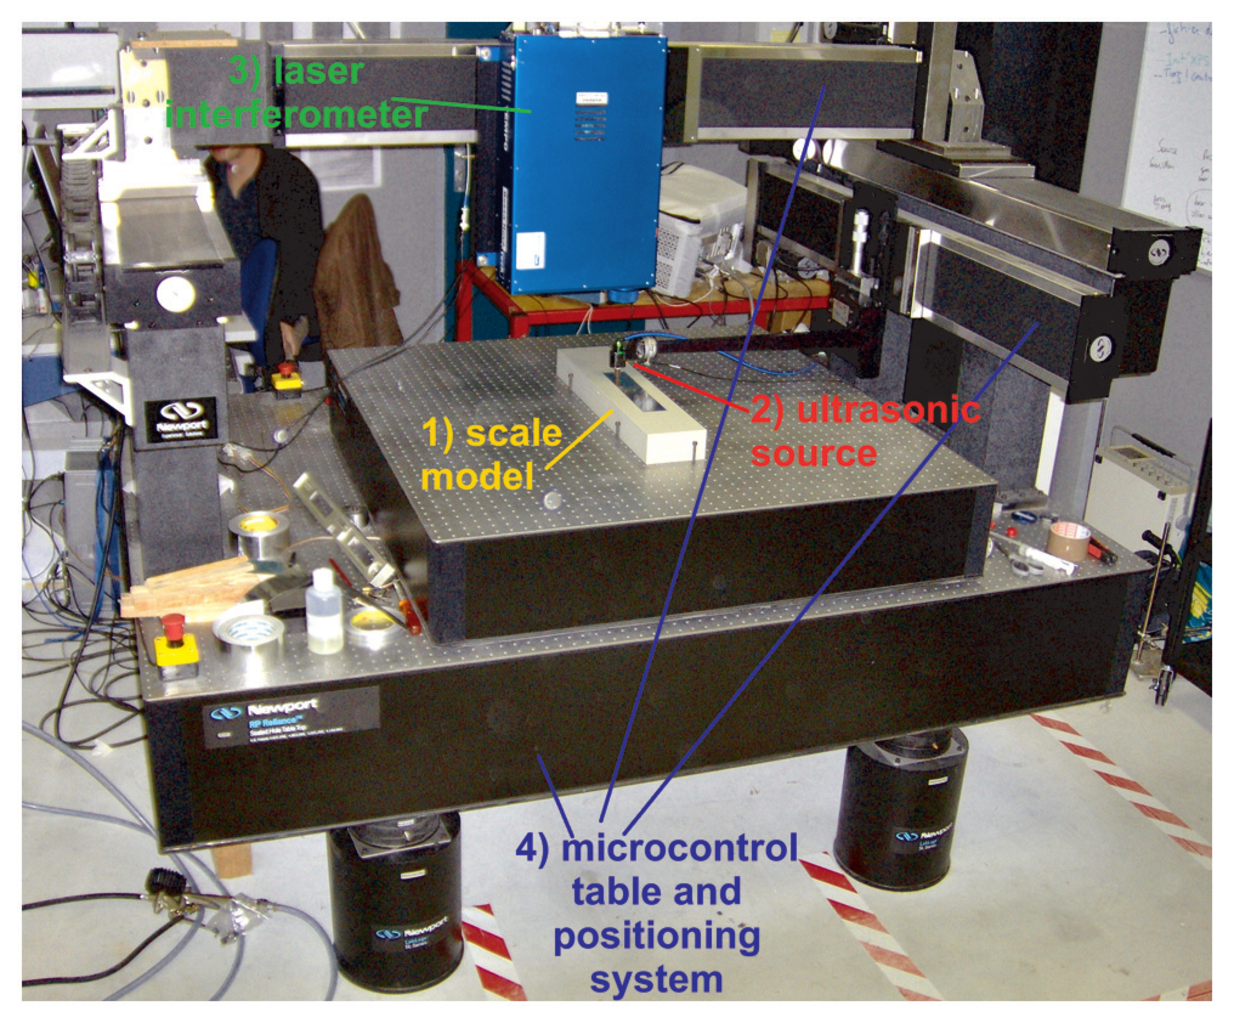
\includegraphics[width=0.75\textwidth]{fig/panel_musc_bench.eps}
	\caption{Photograph of the MUSC ultrasonic laboratory (from \citet{Bretaudeau_FWI_2013} )with its four components: (1) a small-scale model of the underground, (2) an optical table with two automated arms moving above the model, (3) a laser interferometer recording ultrasonic wave propagation	at the model surface,(4) a piezoelectric ultrasonic source generating ultrasonic waves in the model.}
	\label{panel_musc_bench}
\end{figure}

% #### Fig:: panl_multisrcrec
\begin{figure}[!h]
	\centering
	\includegraphics[width=0.75\textwidth]{fig/panel_multisrcrec.eps}
	\caption{Example of multi-source multi-receiver record on the MUSC laboratory for a two-layer model (\bialt).}
	\label{panel_multisrcrec}
\end{figure}

\begin{figure}[!h]
	\centering
	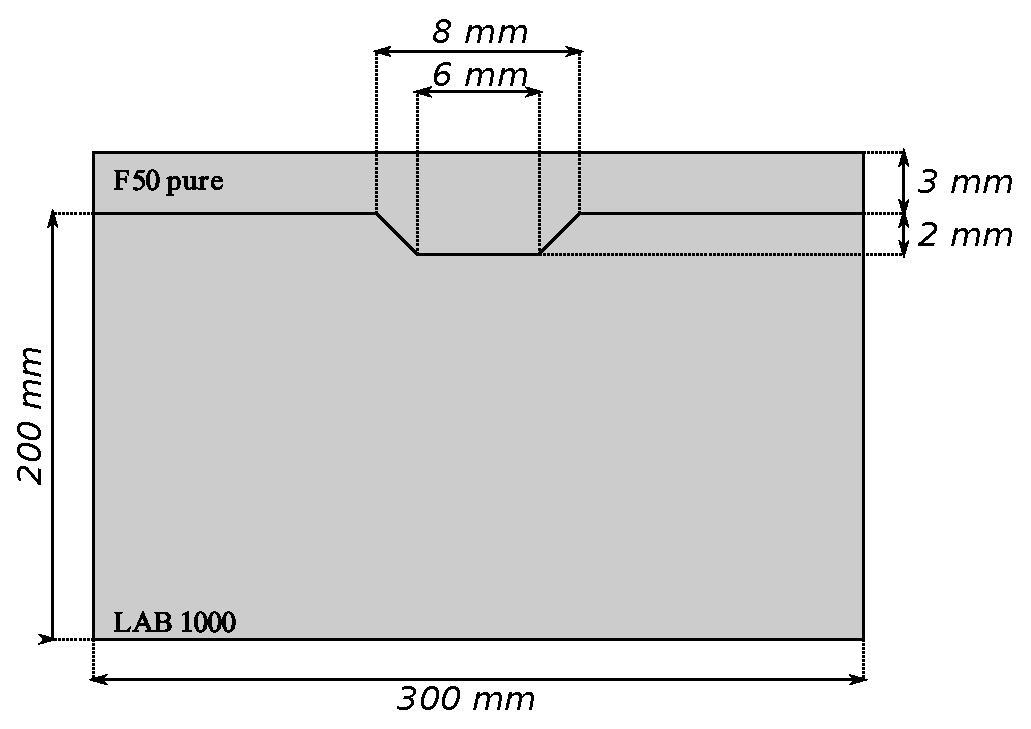
\includegraphics[width=0.75\textwidth]{fig/bialt_model.eps}
	\caption{Schematic representation of the so-called \bialt model.}
	\label{panel_bialt_model}
\end{figure}

\begin{figure}[!h]
	\centering
	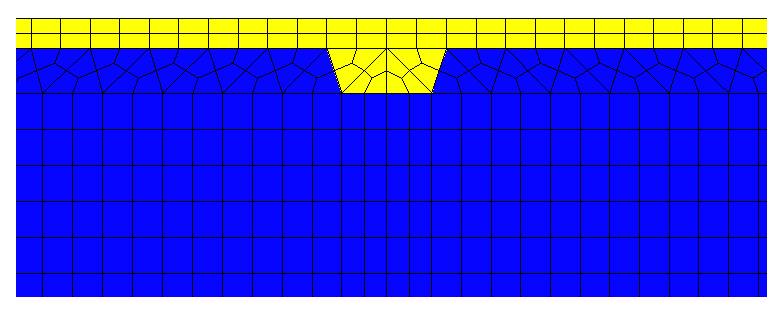
\includegraphics[width=0.75\textwidth]{fig/bialt-mesh.eps}
	\caption{Zoom in the mesh of the \bialt model used for numerical modeling.}
	\label{panel_bialt_mesh}
\end{figure}

% #### Fig:: panel_bialt_2d3d
\begin{figure}[!h]
	\centering
	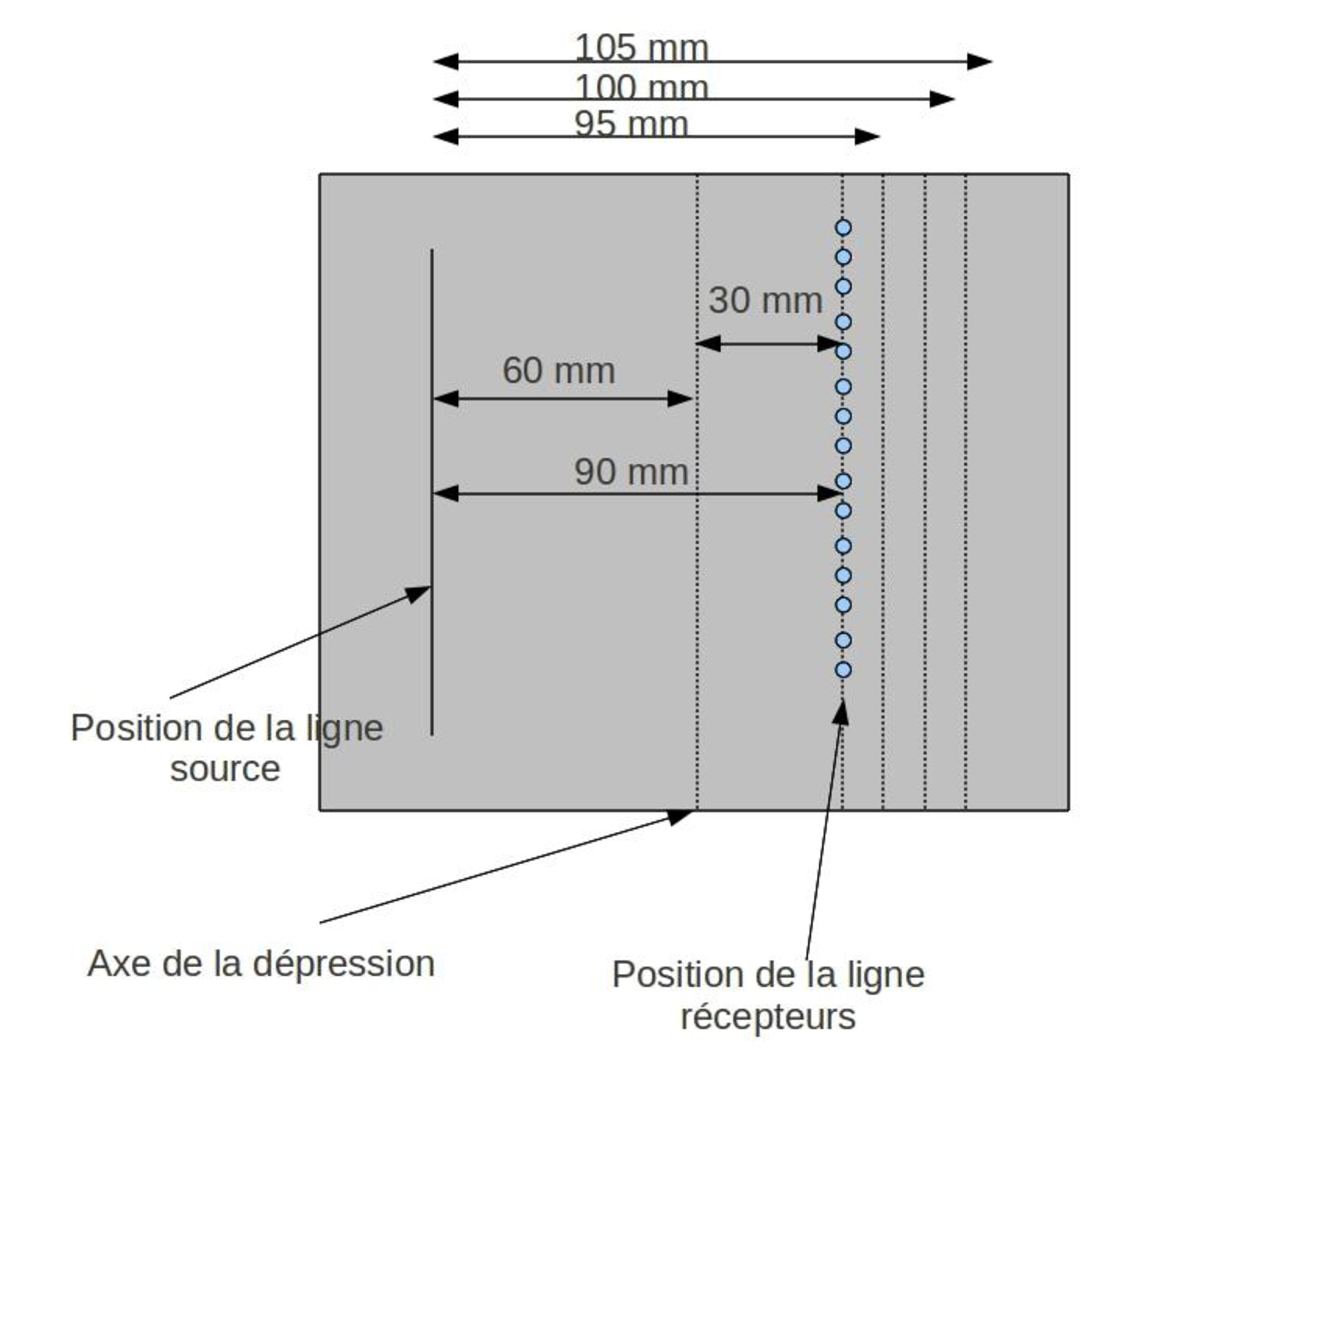
\includegraphics[width=0.75\textwidth]{fig/amplitude_acqui_principle.eps}
	\caption{Schematic representation of the acquisition geometry used to generate experimental line-source, \textit{i.e.} an equivalent of cylindrical source use in two-dimensional modeling. Black triangle and red circle represent receivers and sources, respectively.}
	\label{amplitude_acqui_principle}
\end{figure}

\begin{figure}[!h]
	\centering
	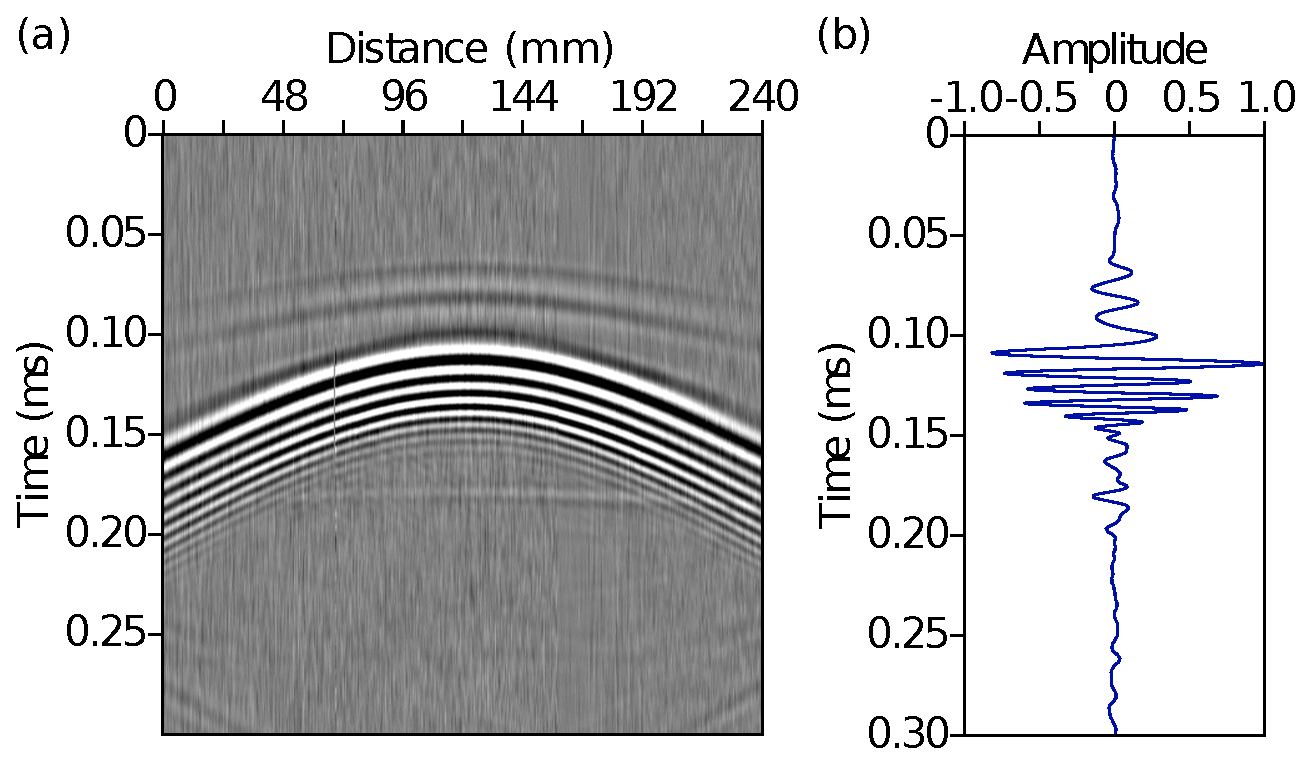
\includegraphics[width=0.75\textwidth]{fig/amplitude_stack_principle.eps}
	\caption{(a,b) Numerical modeling. (a) Resulting seismogram at one receiver position for the experimental line-source. (b) Comparison between point-source response in red (central trace of (a)) , weighted stack response of(a) in green and line-source response from \twod modeling in blue. (c,d) Same as (a) and (b) but for experimental modeling.}
	\label{amplitude_stack_principle}
\end{figure}

\begin{figure}[!h]
	\centering
	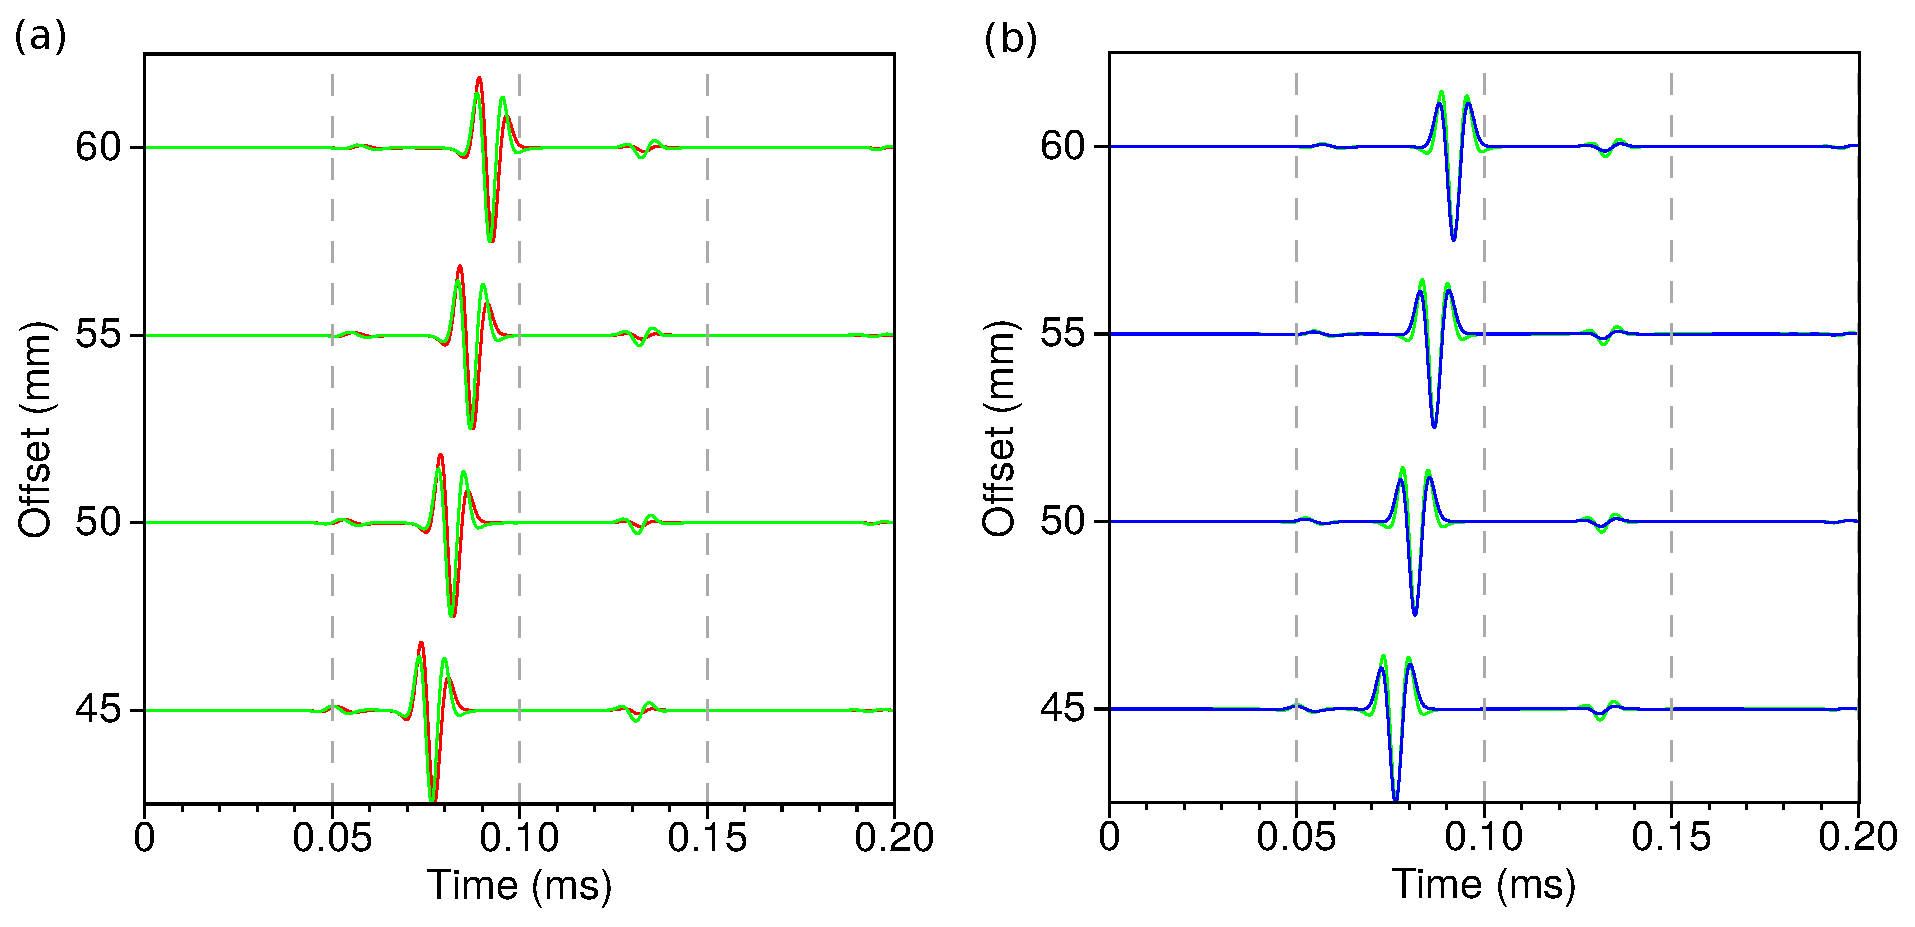
\includegraphics[width=0.75\textwidth]{fig/trans2d3d.eps}
	\caption{(a,b) Numerical modeling. (a) Comparison between synthetic seismograms for a point-source (red) and for a line source (green), for 45, 50, 55 and 60 mm source-receiver offsets respectively. (b) Comparison between synthetic seismograms for a line-source (green), and a point-source response corrected from geometrical spreading (blue) for same source-receiver offsets as (a) using the hybrid method with ratios $r=0.35$, $r=0.40$, $r=0.45$ and $r=0.50$ for offsets $45$, $50$, $55$ and $60\ mm$, respectively . (c,d) Same as (a) and (b) for experimental modeling. The light-purple dotted lines pick $PSv$-wavefront.}%\textbf{cc} gives the correlation factor between line-source and point-source responses.}
	\label{panel_amplitude_sem}
\end{figure}

% #### Fig:: panel_srcest_2d_mean
\begin{figure}[!h]
	\centering
	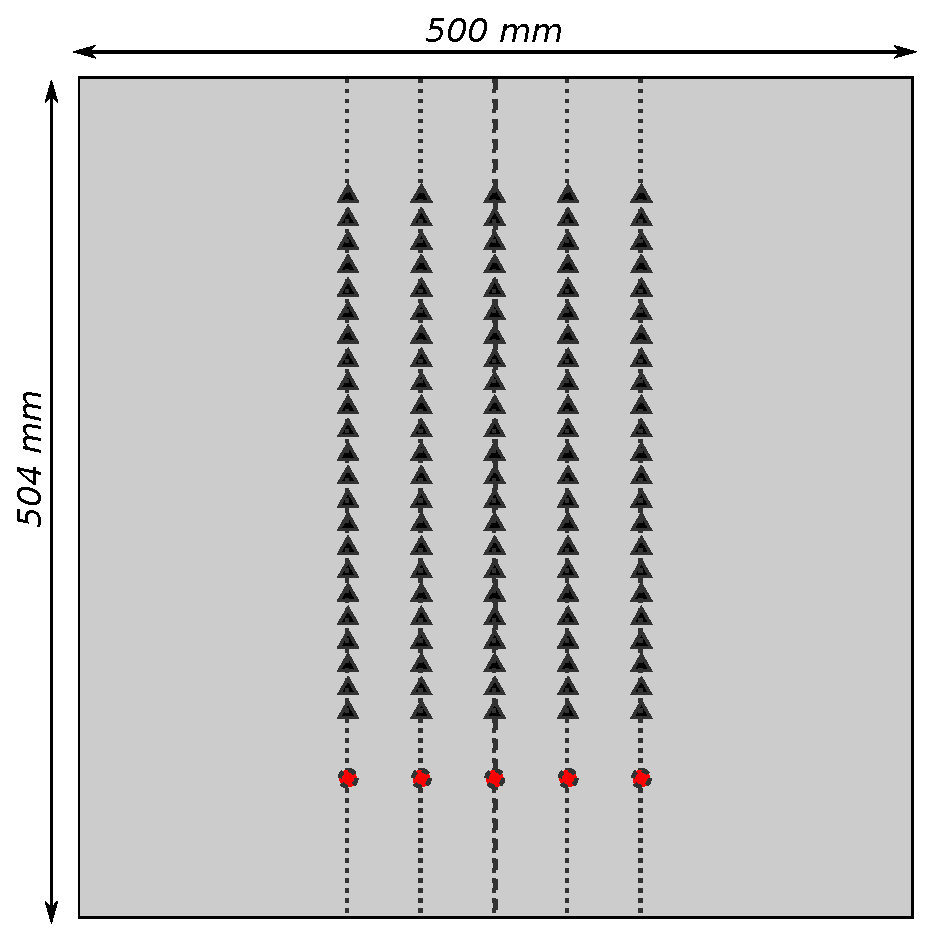
\includegraphics[width=0.75\textwidth]{fig/reproducibility_acqui_principle.eps}
	\caption{Schematic representation of the acquisition geometry used to assess the data reproducibility using the MUSC laboratory. Black triangle and red circle represent receivers and sources, respectively.}
	\label{reproducibility_acqui_principle}
\end{figure}

\begin{figure}[!h]
	\centering
	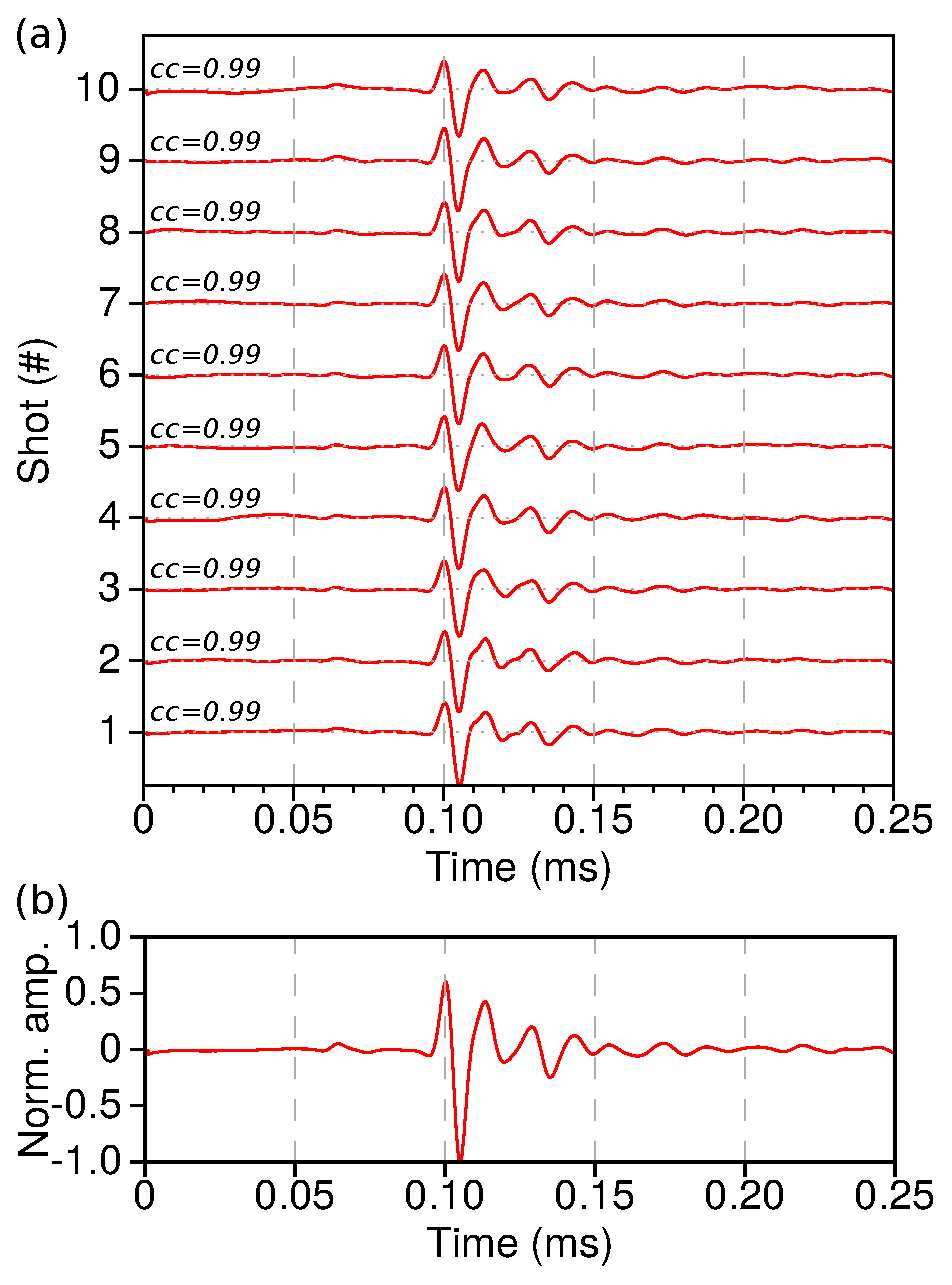
\includegraphics[width=0.75\textwidth]{fig/musc_F50_CT.eps}
	\caption{Central trace for each of the ten analogical experiment compared to a mean central trace (green). \textbf{cc} gives the correlation coefficient between the compared traces.}
	\label{panel_central_traces_cc}
\end{figure}

\begin{figure}[!h]
	\centering
	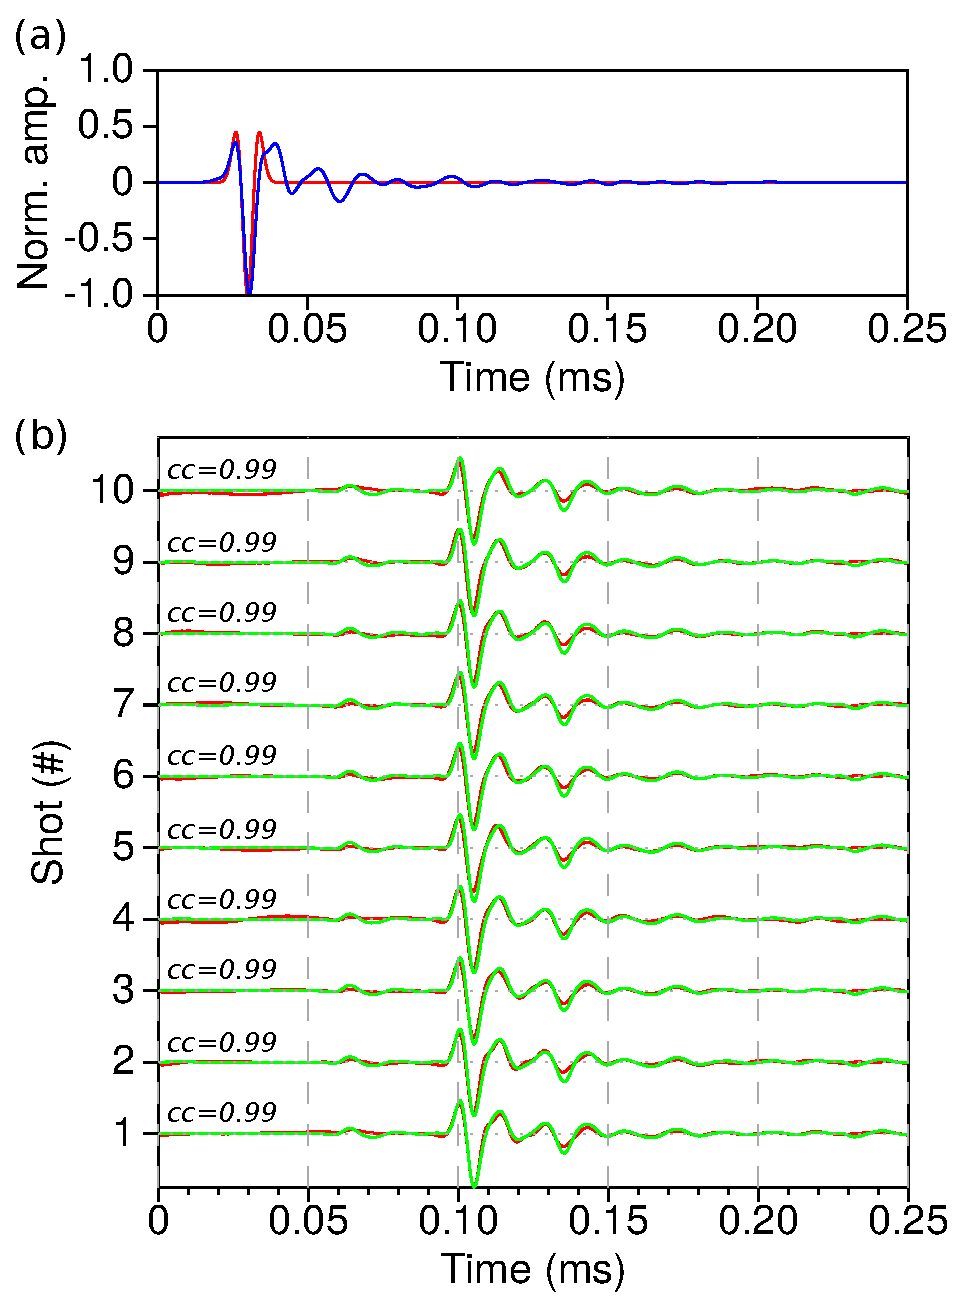
\includegraphics[width=0.75\textwidth]{fig/spec_F50_CT_COMP.eps}
	\caption{(a) Comparison between theoretical Ricker source ($f_{0}=100\ kHz$, $t_{0}=0.03\ ms$) send to the piezoelectric transducer (dashed red line) and the effective source for the homogeneous \textit{F50 pure} model (blue line). (b) Comparison between experimental central traces and numerical ones using the effective source instead theoretical one. \textbf{cc} gives the correlation coefficient between experimental and synthetic traces.}
	\label{panel_srcest_2d_mean_comp}
\end{figure}

% #### Fig:: panel_bialt_model


\begin{figure}[!h]
	\centering
	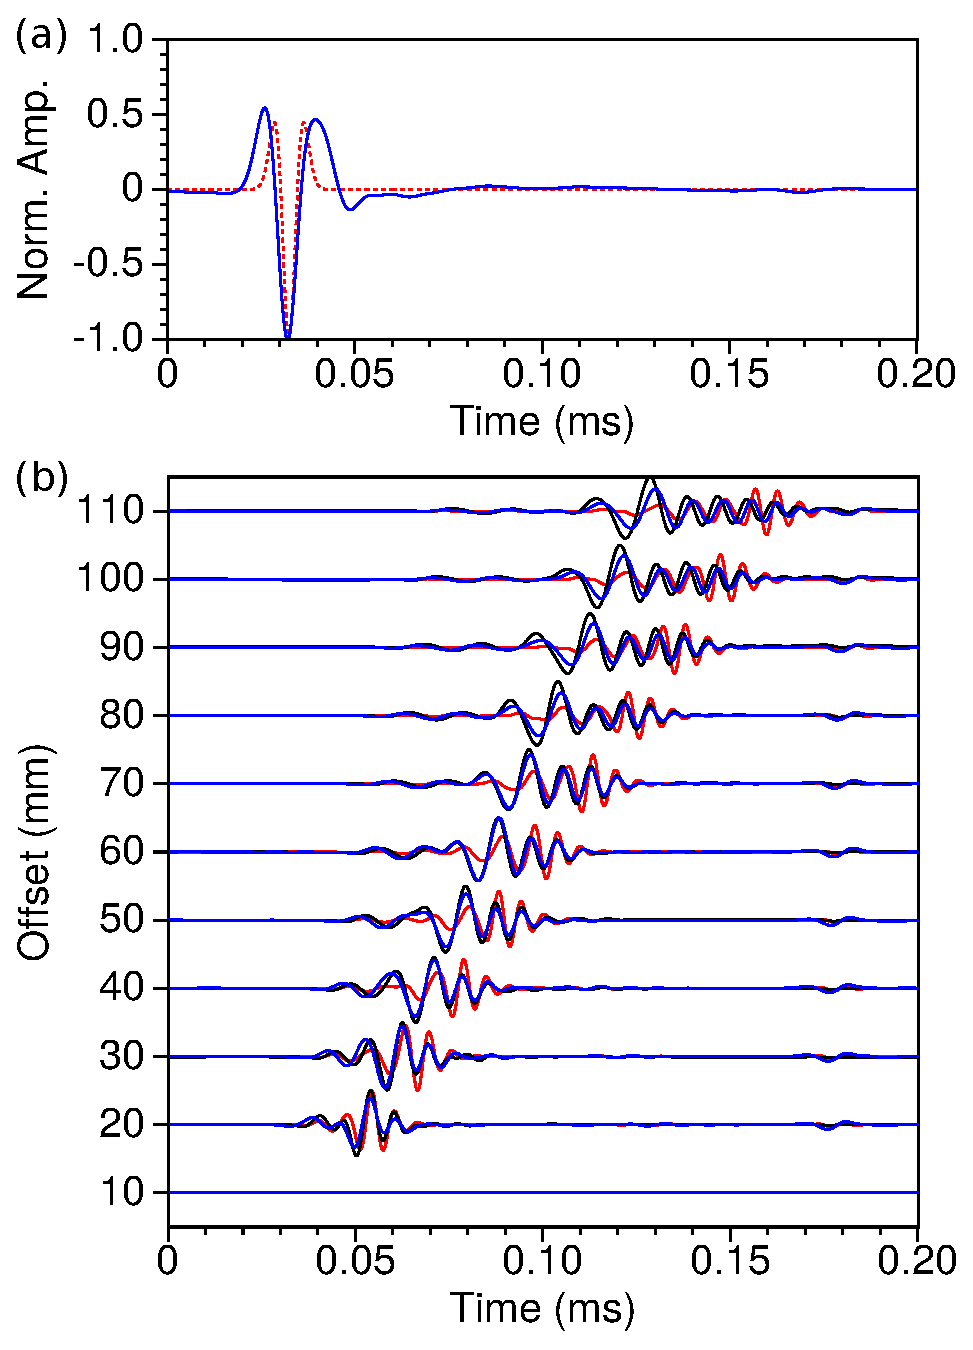
\includegraphics[width=0.75\textwidth]{fig/panel_bialt_lswe.eps}
	\caption{(a) Comparison between theoretical Ricker source ($f_{0}=75\ kHz$, $t_{0}=0.03\ ms$) send to the piezoelectric transducer (dashed red line) and the effective source for the \bialt model (blue line). (b) Comparison between experimental central traces (black), numerical traces using theoretical source (red) and numerical traces using the effective source (blue). }
	\label{blind-test}
\end{figure}

\clearpage
\newpage

\subsection*{Tables}

\begin{table}[!ht]
	\centering
	\begin{tabular}{cccccc}
		\hline
		material & Field experiment scale & MUSC experiment scale & scales ratio  \\
		\hline
		P waves velocity & $\mathrm{V_{p 0}}$ & $\mathrm{V_{p 0}}$  & 1  \\
		S waves velocity & $\mathrm{V_{s 0}}$ &  $\mathrm{V_{s 0}}$ & 1   \\
		Time & $\mathrm{T_{0}}$    & 0.001 $\mathrm{T_{0}}$ & 0.001  \\
		frequency   & $\mathrm{F_{0}}$  & 1000 $\mathrm{F_{0}}$ & 1000  \\
		Distance   & $\mathrm{D_{0}}$  & 0.001 $\mathrm{D_{0}}$ & 0.001   \\
		Wavelength   & $\mathrm{D_{0}}$ & 0.001 $\mathrm{D_{0}}$ & 0.001  \\
		\hline
	\end{tabular}
	\caption{ example of possible scales ratio between field experiments and MUSC experiments when considering a ratio equal to 1 for the density and Quality factor.}
	\label{epoxy-resin}
\end{table}

\begin{table}[!ht]
	\centering
	\begin{tabular}{cccccc}
		\hline
		material & Field experiment scale & MUSC experiment scale & scales ratio  \\
		\hline
		P waves velocity & $\mathrm{V_{p 0}}$ & $\mathrm{2V_{p 0}}$  & 2  \\
		S waves velocity & $\mathrm{V_{s 0}}$ &  $\mathrm{2V_{s 0}}$ & 2   \\
		Time & $\mathrm{T_{0}}$    & 0.001 $\mathrm{T_{0}}$ & 0.001  \\
		frequency   & $\mathrm{F_{0}}$  & 2000 $\mathrm{F_{0}}$ & 2000  \\
		Distance   & $\mathrm{D_{0}}$  & 0.001 $\mathrm{D_{0}}$ & 0.001   \\
		Wavelength   & $\mathrm{D_{0}}$ & 0.001 $\mathrm{D_{0}}$ & 0.001  \\
		\hline
	\end{tabular}
	\caption{ example of possible scales ratio between field experiments and MUSC experiments when considering a ratio equal to 2 for the density and Quality factor.}
	\label{epoxy-resin}
\end{table}


\begin{table}[!ht]
	\centering
	\begin{tabular}{cccccc}
		\hline
		material & $\mathrm{V_{P}\ (m/s)}$ & $\mathrm{V_{S}\ (m/s)}$ & $\mathrm{V_{R}\ (m/s)}$ & $\mathrm{\rho\ (kg/m^{3})}$ & $\mathrm{Q}$ \\
		\hline
		Aluminum & 5630 & 3225 & --   & 2700 & --  \\
		F50 pure  & 2300 & 1030 & 965  & 1300 & 30  \\
		F50 200\% & 2820 & 1425 & 1328 & 1766 & --  \\
		F50 240\% & 2968 & 1496 & 1388 & 1822 & --  \\
		LAB1000   & 2850 & 1400 & 1310 & 1500 & 75  \\
		\hline
	\end{tabular}
	\caption{Physical properties of some materials used to build small scale models. $\mathrm{V_{P}}$, $\mathrm{V_{S}}$ and $\mathrm{V_{R}}$ are the P-wave velocity, S-wave and the Rayleigh wave velocity, respectively. $\rho$ is the density and $\mathrm{Q}$ is the quality factor.}
	\label{epoxy-resin}
\end{table}

% \begin{table}[!ht]
%	\centering
%	\begin{tabular}{|l|lcr|}
%		
%		\hline
%		Distance               & $d_{real}\ (m)$            & $\rightarrow$ & $k^{-1}d_{reduc}\ (mm)$ \\
%		Wavelength             & $\lambda_{real}\ (m)$      & $\rightarrow$ & %$k^{-1}\lambda_{reduc}\ (mm)$ \\
%		Time                   & $t_{real}\ (s)$            & $\rightarrow$ & $k^{-1}t_{reduc}\ (ms)$ \\
%		Velocity               & $V_{real}\ (m.s^{-1})$     & $\rightarrow$ & $V_{reduc}\ (m.s^{-1})$ \\
%		Density                & $\rho_{real}\ (kg.m^{-3})$ & $\rightarrow$ & $\rho_{reduc}\ (kg.m^{-3})$ \\
%		Quality factor         & $Q_{real}$                 & $\rightarrow$ & $Q_{reduc}$ \\
%		Particle displacement & $a_{real}\ (m)$            & $\rightarrow$ & $k^{-1}a_{reduc}\ (mm)$ \\
%		Particle velocity     & $c_{real}\ (m.s^{-1})$     & $\rightarrow$ & $c_{reduc}\ (m.s^{-1})$ \\
%		\hline
%	\end{tabular}

%	\caption{Scale ratio between viscoelastic parameters at the real scale and at a scale reduced by a coefficient $k$ (after \citet{Bretaudeau_SSM_2011}).}
%	\label{scale-ratio}
%\end{table}

%\begin{table}[!ht] 
%	\centering
%	\begin{tabular}{lcccc}
%		\hline
%		\qquad & 90 mm & 95 mm & 100 mm & 105 mm \\
%		\hline
%		$cc1_{init}$  & 0.702 & 0.725 & 0.728 & 0.728 \\
%		$rms1_{init}$ & 0.794 & 0.760 & 0.762 & 0.774 \\
%		\hline
%		$cc1_{final}$  & 0.940 & 0.953 & 0.951 & 0.949 \\
%		$rms1_{final}$ & 0.358 & 0.317 & 0.325 & 0.343 \\
%		\hline
%		\hline
%		$cc2_{init}$  & 0.954 & 0.987 & 0.988 & 0.988 \\
%		$rms2_{init}$ & 0.304 & 0.162 & 0.155 & 0.154 \\
%		\hline
%		$cc2_{final}$  & --   & --    & --    & --    \\
%		$rms2_{final}$ & --   & --    & --    & --    \\
%		\hline
%	\end{tabular}
%	\caption{.}
%	\label{cc-rms}
%\end{table}

\clearpage
\newpage

\bibliographystyle{seg}  % style file is seg.bst
%\bibliography{/media/pageotd/1581-58C8/Work/git-repository//TR-VIBRIS/tail/bibvibris}
\bibliography{bibvibris,bibvibris_Dona,bibvibris-Dona,references}

\end{document}
